\documentclass[../../main.tex]{subfiles}

\begin{document}
\problem{22}
\begin{wts}
What is the largest possible source port number?  
\end{wts}
\providecommand{\xn}{\{x_n\}}
\providecommand{\buck}{\mathcal{B}}
\providecommand{\queue}{\mathcal{Q}}

\begin{proof}
    Consider the following graphic,\\
    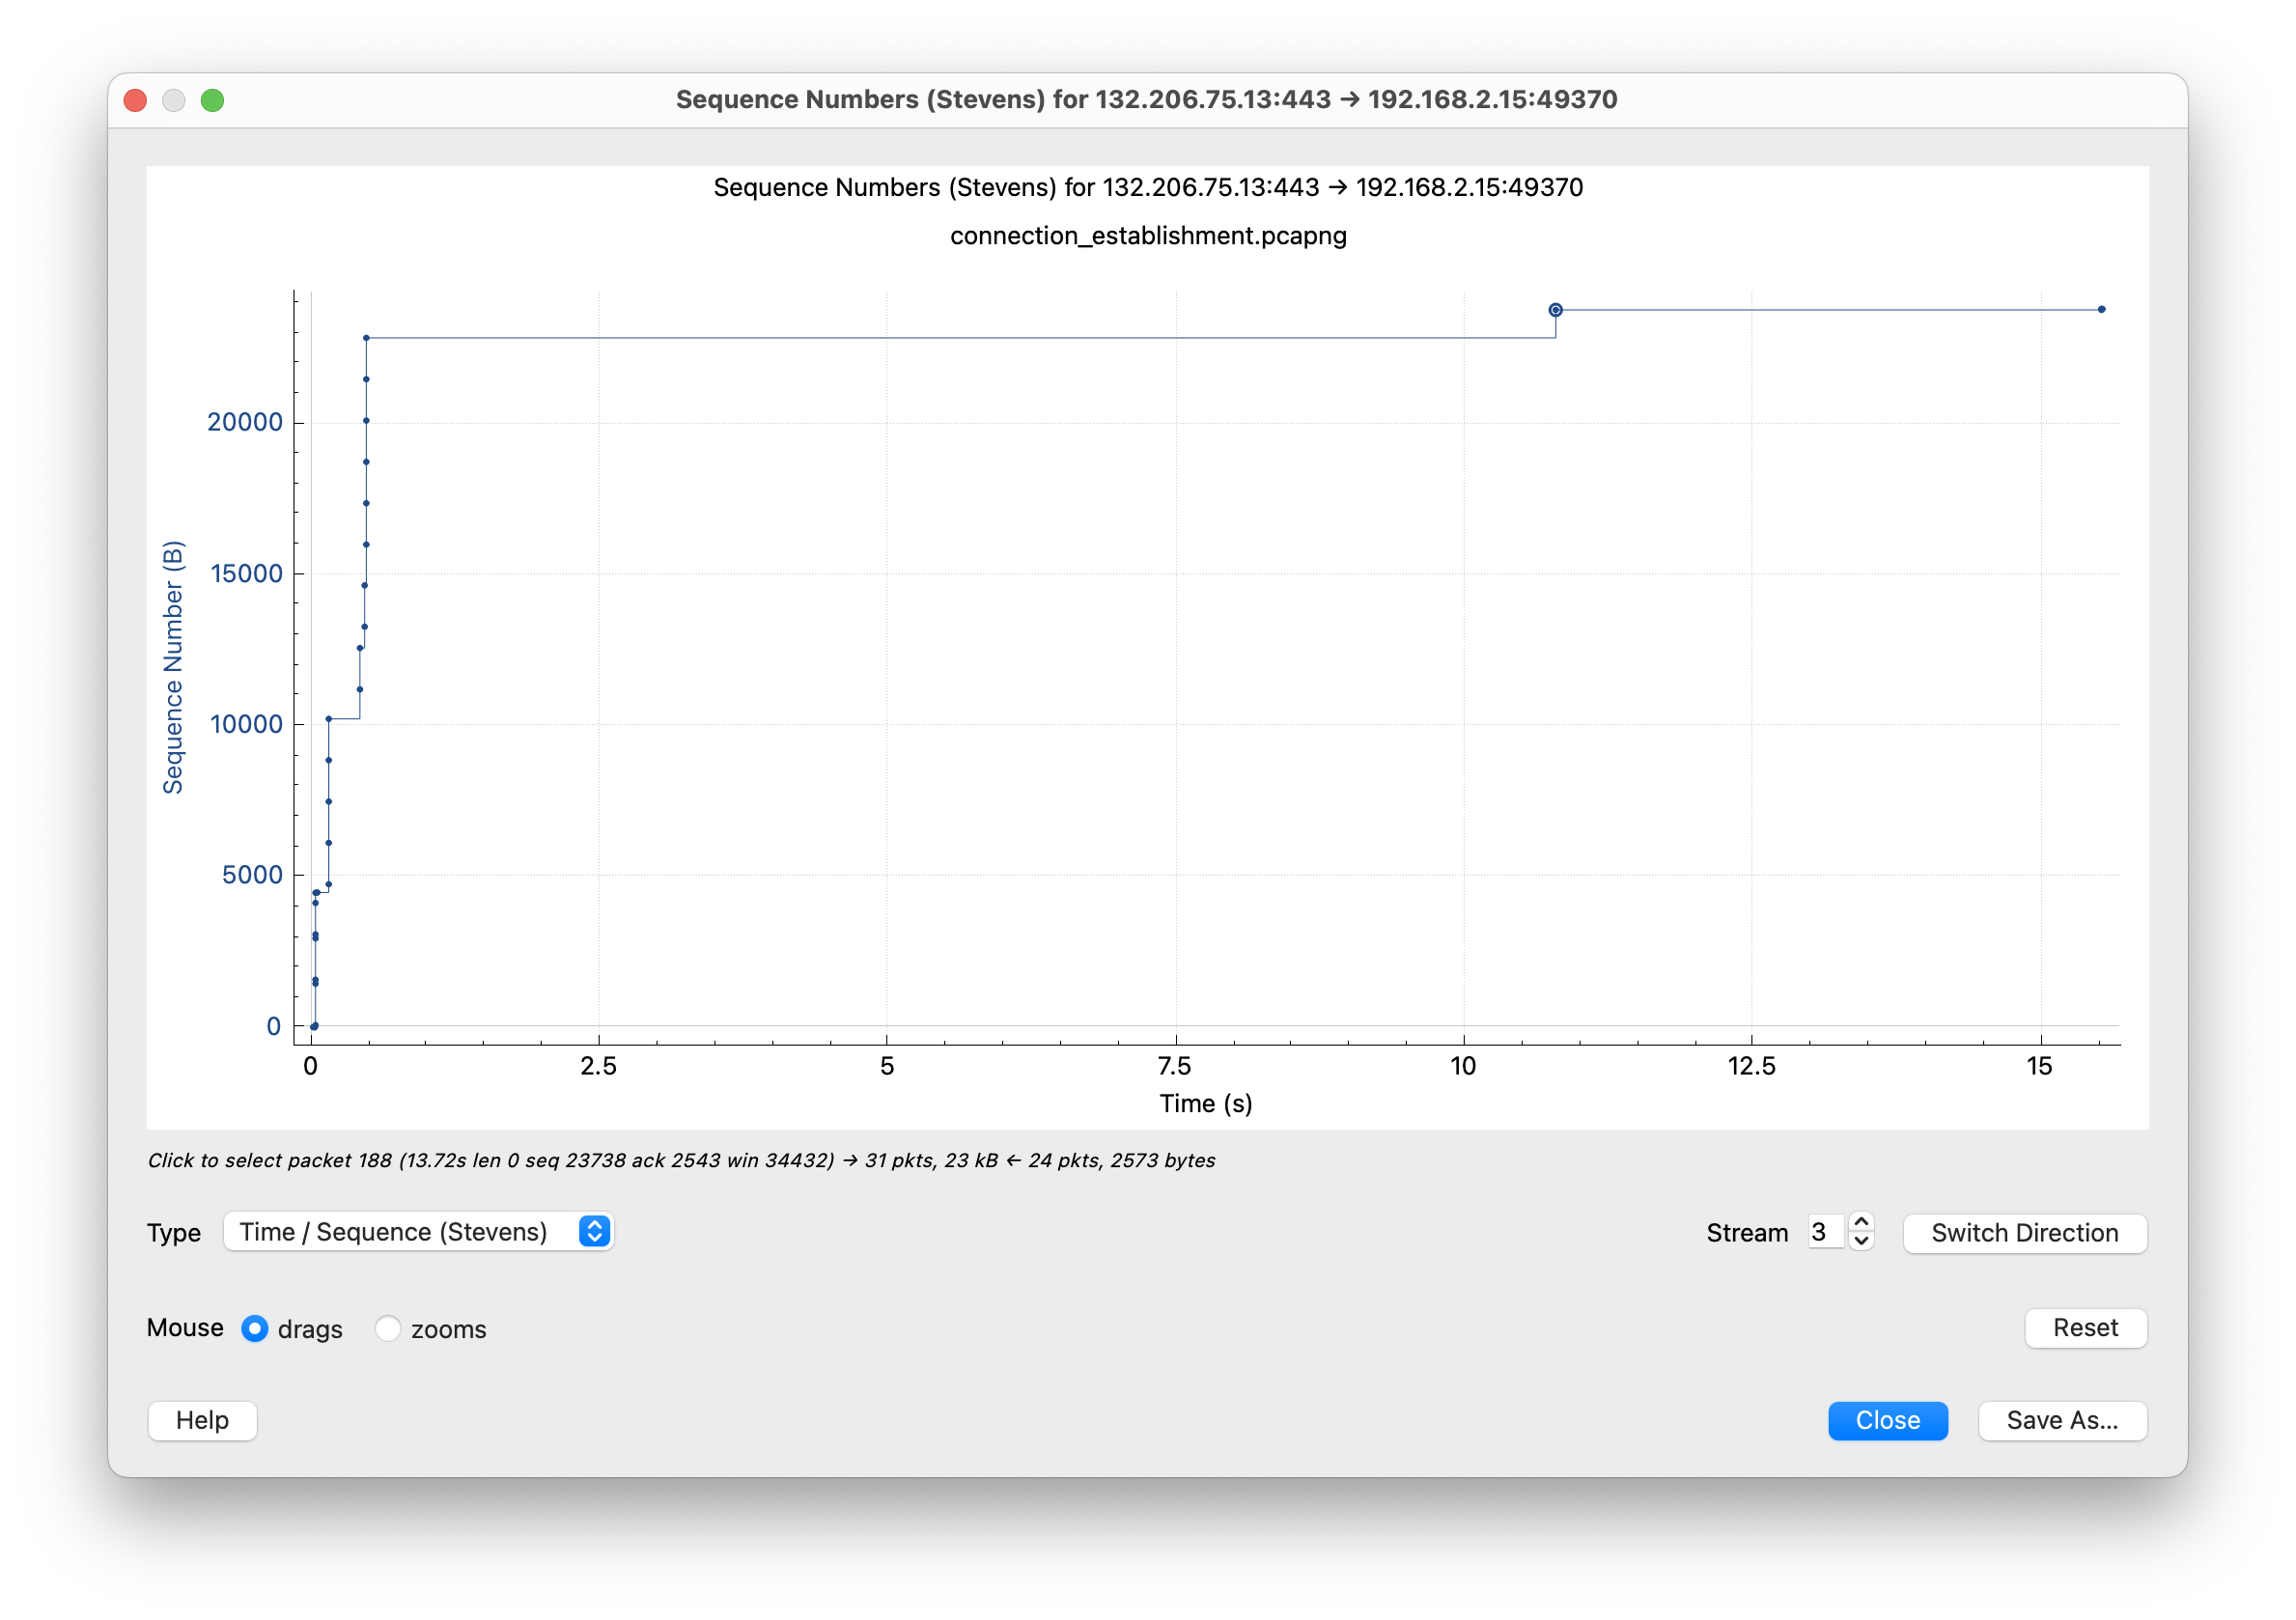
\includegraphics[width=\textwidth]{subfiles/images/connection_bytestream_plot_Q19_server_to_client.png}
    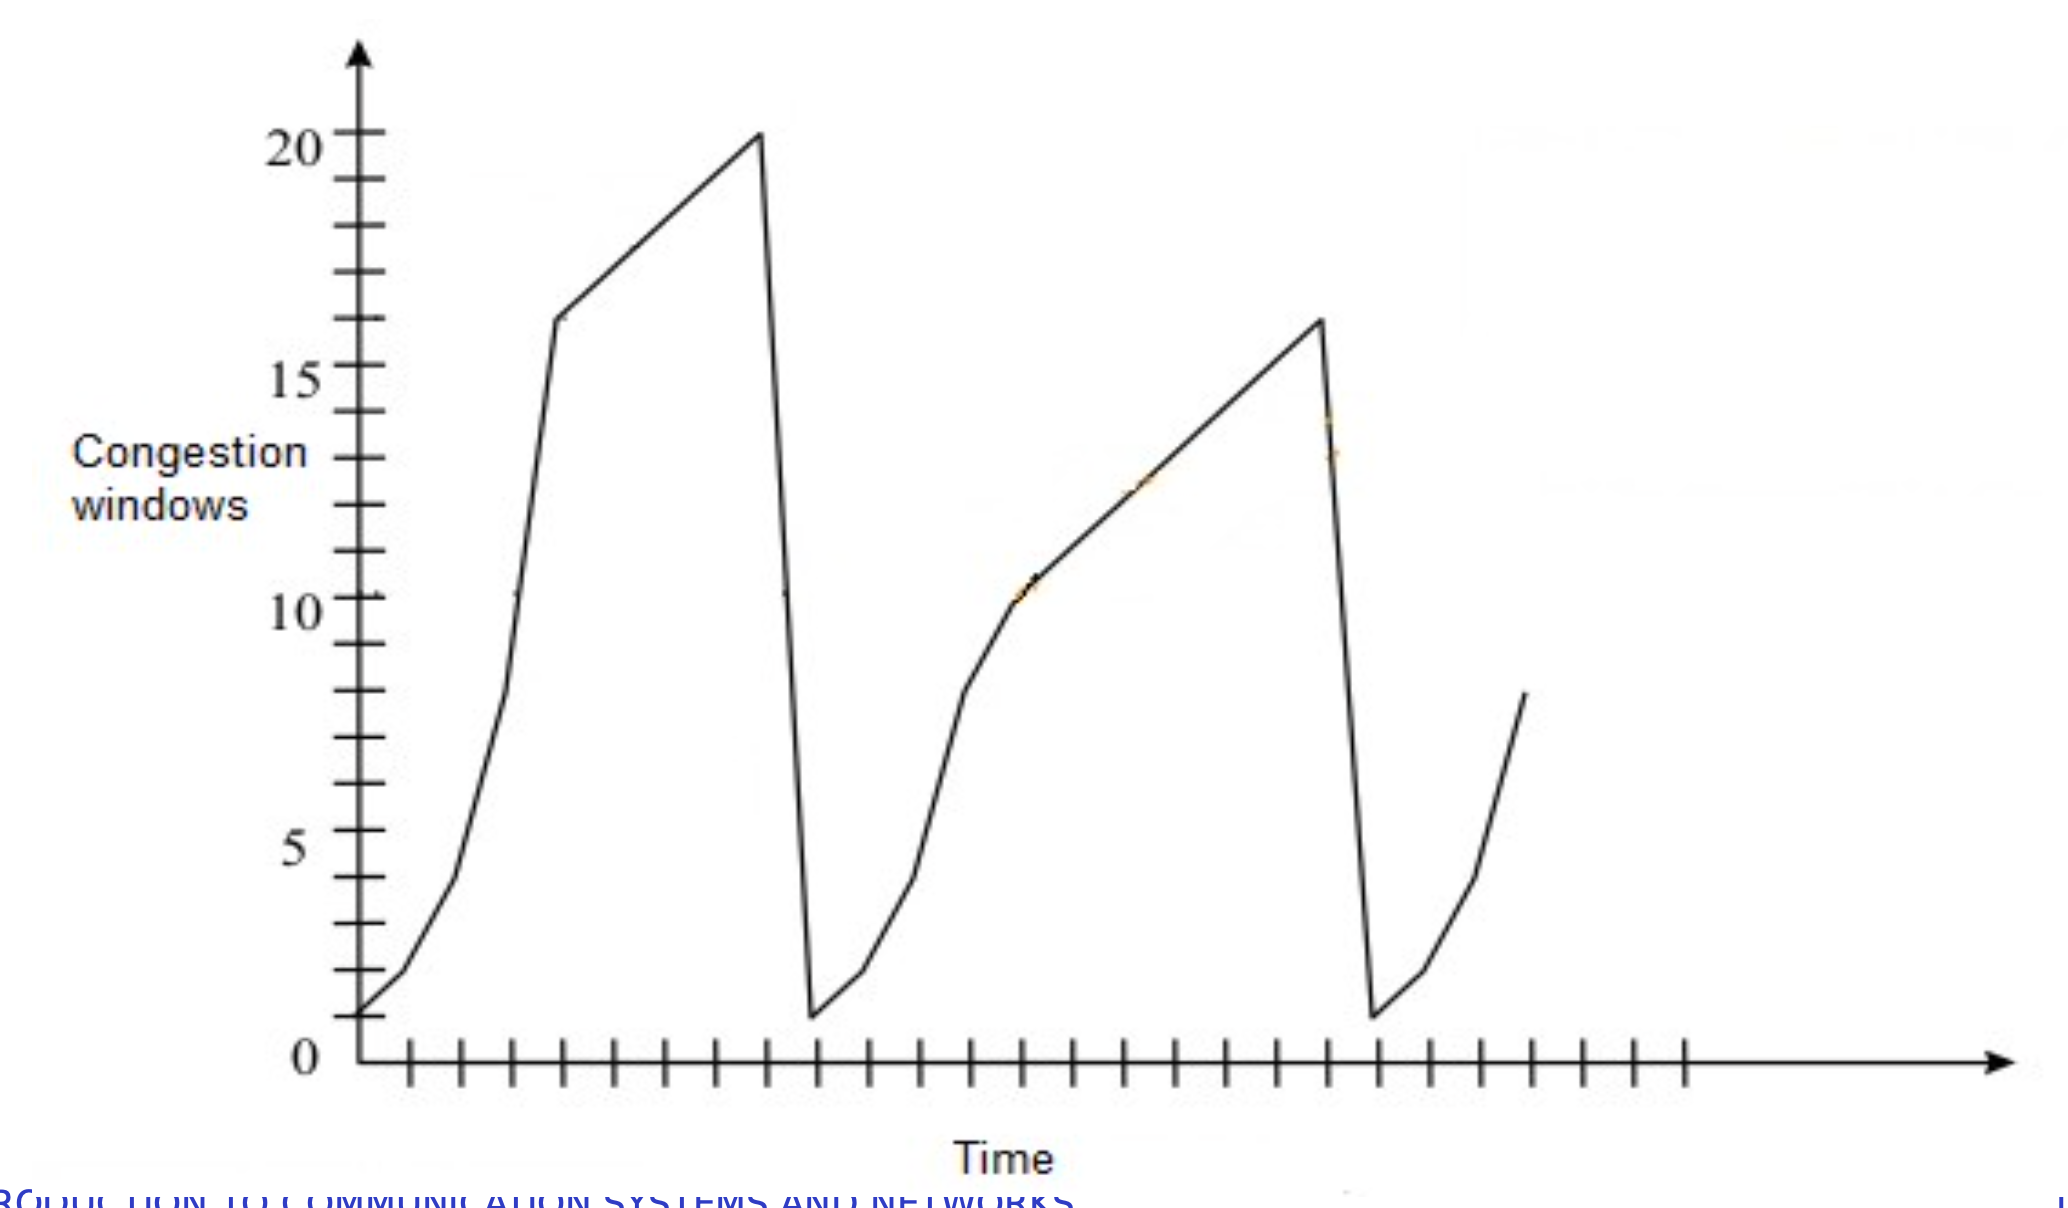
\includegraphics[width=\textwidth]{subfiles/images/part3_q19_window_graphic.png}
    We first argue that the question is ill-posed. If the queue size is infinite, then the bucket size can be $0$, (hereinafter denoted by $\mathcal{B}\geq 0$. Clearly, there are two variables to consider, and one cannot determine the minimum necessary (and hence sufficient) bucket size $\buck$ from $r\geq 1$ alone.\\
    
    Furthermore, the question is vague in the sense that there is a lack of information on the timing of the tokens within an interval. Suppose the system is at equilibrium with $b(t_0)=\buck$, and let $r=1>0$, and fix $a(t_0)=B+1$. This arrival of packets $a(t)$ can occur entirely before, partially before, partial after, and entirely after the token drop of $r=1$. The bucket spills over in the first case, but withstands the inflows in all others.\\
    
    To this, our answer will make several assumptions.
    \begin{itemize}
        \item First, all tokens arrive at the same time at integral numbers of $t_0$, or at $t=1,\ldots, L$ (we will discard the continuous time notation from now on),
        \item Second, the maximum queue size permissible denoted by $\queue$ must satisfy
        \[\queue = \max_{i\in[0,L]}\biggl\{q(i)\biggr\}=0\]
        \item Third, we assume the bucket temporarily holds all of the token drops $r$ regardless of its size, for one interval, but it must not retain a balance strictly greater than $\buck$ after all packet arrivals
        \item Fourth, we assume that all token drops occur strictly prior to any arrival of packets this will impose the strictest of conditions
    \end{itemize}
    From the definition of the queue $q(i)$,
    \begin{equation}\label{queue equation}
        q(i)=\max\biggl\{a(i)+q(i-1)-b(i-1)-r,0\biggr\}
    \end{equation}
    Notice that $Q=0$ is equivalent to \[a(i)+q(i-1)-b(i)-r\leq 0\]
    for every $i\in[0,L]$. Indeed, suppose $Q=0$ holds, it follows from \eqref{queue equation} that $q(i)\geq 0$ at every $i$. Then,
    \[\forall i\geq 0,\,Q\geq q(i)\geq 0\iff q(i)=0\]
    so that for every $i\geq 0$\[a(i)+q(i-1)-b(i)-b(i)-r\leq q(i)\leq Q=0\] Notice that $0$ is a lower bound, (from Equation \eqref{queue equation}) so
    \[0\leq q(i)\leq \min_{i\geq 0}q(i)\leq \max_{i\geq 0}q(i)=Q\]
    and to show the contrapositive, suppose $Q>0$ then there exists an $i>0$ (without loss of generality) with
    \begin{align*}
        q(i)&=Q>0\\ q(i)&=\max\{a(i)-q(i-1)-b(i)-r,0\}\\
        &=a(i)-q(i-1)-b(i)-r>0
    \end{align*}
    Now suppose $b_0=\buck$ and $r\geq 1$ are fixed, we will show
    \begin{equation}\label{balance equation}
    b_k=b_0 + \min\biggl\{0,\min_{1\leq N\leq k}\sum^N_{\alpha = 1}\Delta(k-\alpha)\biggr\}
    \end{equation}
    where $\Delta(j)=r-a(j)$. When $k=0$ it is trivial, so suppose \eqref{balance equation} holds for $k\in [0,A]$, and by strong induction
    \begin{align*}
        b_{A+1} &= \min\biggl\{b_0,b_0 + \Delta(A+1 -1),\biggl(\min_{1\leq N\leq A}b_0 + \sum^N_{\alpha = 1}\Delta(A-\alpha)\biggr)+\Delta(A+1-1)\biggr\}\\
        &= \min\biggl\{b_0,b_0 + \Delta(A+1 -1),\biggl(\min_{1\leq N\leq A}b_0 + \sum^N_{\alpha = 1}\Delta(A+1-(\alpha+1))\biggr)+\Delta(A+1-1)\biggr\}\\
        &= \min\biggl\{b_0,b_0 + \Delta(A+1 -1),\biggl(\min_{1\leq N\leq A}b_0 + \sum^{N+1}_{\alpha = 2}\Delta(A+1-\alpha)\biggr)+\Delta(A+1-1)\biggr\}\\
        &= \min\biggl\{b_0,b_0+\biggl(\min_{1\leq N\leq A+1} \sum^{N}_{\alpha = 1}\Delta(A+1-\alpha)\biggr)\biggr\}\\
        &= b_0 + \min\biggl\{0,\min_{1\leq N\leq A+1} \sum^{N}_{\alpha = 1}\Delta(A+1-\alpha)\biggr\}
    \end{align*}
    where we used (and the reader can verify)
    \begin{itemize}
        \item $y=\min(a,b)$, if and only if
        \[y\leq a,\,y\leq b\]
        \item $\min(a,\min(a,b)) = \min(a,b)$
        \item $\min(a+c,b+c) = c+\min(a,b)$
    \end{itemize}
    Let $\buck_i$ be the tenatative infimum for permissible bucket sizes to achieve non-negative bucket balances, where $i$ ranges within $[0,L]$. For convenience, $\buck_{i-1}=0$. We claim that we can generate a sequence of tightest lower bounds for $[0,N]\subseteq [0,L]$ with 
    \begin{equation}\label{bucket adjustment}
    \buck_{N+1}=\buck_{N}+\max\biggl\{0,-\Delta(N+1)-\buck_{N}-\min\biggl\{0,\min_{1\leq M\leq N+1}\sum^M_{\alpha=1}\Delta(N+1-\alpha)\biggr\}\biggr\}
    \end{equation}
    Choose $\buck_0$ by invoking the Well-Ordering Property of $\nat$ so that 
    \[\buck_0=\least\biggl\{n\in\nat_0,\,n\geq-\Delta(0)=a(0)-r\biggr\}\]
    as it is clear since $\real$ is Archmedean.\\
    
    Suppose $\buck_0,\buck_1,\ldots,\buck_A$ have been chosen and for each $n\in[0,A]$, and $k\in[0,n]$, with $b_k^n$ denoting the bucket balance at $t=k$ during the $n$-th iteration, and it reads
    \begin{equation}\label{bucket sequence estimate}
        b_k^n\geq -\Delta(k)=a(k)-r,\quad b_0^n = \buck_n
    \end{equation}
    Now let $k=A$, and we wish to show \eqref{bucket sequence estimate} holds for $k+1$ if we take $b^{A+1}_0=\buck_{A+1}$ as defined in \eqref{bucket adjustment}. Indeed, if 
    \[-\Delta(A+1)-\buck_{A}-\min\biggl\{0,\min_{1\leq N\leq A+1}\sum^N_{\alpha=1}\Delta(A+1-\alpha)\biggr\}>0\]
    then
    \begin{equation}\label{induction Bucket Estimate}-\Delta(A+1)>\buck_{A}+\min\biggl\{0,\min_{1\leq N\leq A+1}\sum^N_{\alpha=1}\Delta(A+1-\alpha)\biggr\}\end{equation}
    applying Equation \eqref{balance equation} to Equation \eqref{induction Bucket Estimate} will suffice. If on the contrary \[-\Delta(A+1)-\buck_{A}-\min\biggl\{0,\min_{1\leq N\leq A+1}\sum^N_{\alpha=1}\Delta(A+1-\alpha)\biggr\}\leq 0\]
    we have
    \[-\Delta(A+1)\leq \buck_{A}+\min\biggl\{0,\min_{1\leq N\leq A+1}\sum^N_{\alpha=1}\Delta(A+1-\alpha)\biggr\}\leq 0\]
    and it is clear from Equation \eqref{balance equation} that $\buck_{A+1}=\buck_{A}$ is sufficient, and indeed this is what Equation \eqref{bucket adjustment} does.\\
    
    We can solve for the values of $\buck$ for $r\geq 1$, noting that it is clear from Equation \eqref{bucket adjustment} and \eqref{bucket sequence estimate} that a $\buck=0$ must suffice for $r\geq 6$. In symbols,
    \begin{equation}\label{easy exercise}r\geq \norm{a(t)}_\infty\implies \buck=\sup\biggl\{\buck_N,\,N\in[0,L]\biggr\}=0\end{equation}
    The proof of \eqref{easy exercise} is left as an easy exercise for the reader. (Hint: Look at the values of $\Delta$). Using a few lines of code, we get
    \begin{center}
    \captionof{table}{\textbf{r and infimum bucket size}}
    \begin{tabularx}{\textwidth}{l r r r r r}
    \cmidrule[0.75pt](r){1-6}\addlinespace[0.2em]
    
    r&1&2&3&4&5\tabularnewline
    $\buck$&10&7&4&2&1\tabularnewline
    
    \cmidrule[0.75pt](r){1-6}\addlinespace[0.2em]
    \end{tabularx}\label{BucketSizes}
\end{center}
and $\buck=0$ for $r\geq 6$.
\end{proof}

\end{document}